The interaction of different particles with the nuclei or the
electrons in the gas of the TPC produces different patterns of the 2D
projection of the initial 3D particle trajectory.  These cluster shape
observables are useful to discriminate different ionizing
particles. In particular, they were used to select a pure sample of
nuclear recoil candidates produced by the interaction of the neutrons
originating from the \ambe source and to identify various sources of
backgrounds. The main cluster shape observables are described in the
following:

\begin{itemize}
  \item \textit{projected length and width:~} a SVD on the $x \times
    y$ matrix of the pixels belonging to the supercluster is
    performed. The eigenvectors found can be interpreted as the
    directions of the two axes of an ellipse in 2D. The eigenvalues
    represent the magnitudes of its semiaxes: the major one is defined
    as \textit{length}, $l$ the minor one as \textit{width},
    $w$. These are well defined for elliptic clusters, or for long and
    straight tracks. The directions along the major and the minor axis
    are defined as \textit{longitudinal} and \textit{transverse} in
    the following. The longitudinal and transverse supercluster
    profiles, for the cosmic ray track candidates shown as an example
    in Fig.~\ref{fig:super_clusters2} (bottom) are shown in
    Fig.~\ref{fig:profiles}. The longitudinal profile shows the
    typical pattern of energy depositions in clusters, while the
    transverse profile, dominated by the diffusion in the gas, shows a
    Gaussian shape. It has to be noted that the cluster sizes
    represent only the projection of the 3D track in the TPC on the 2D
    $x$--$y$ plane;

    \begin{figure}[ht]
      \begin{center}
        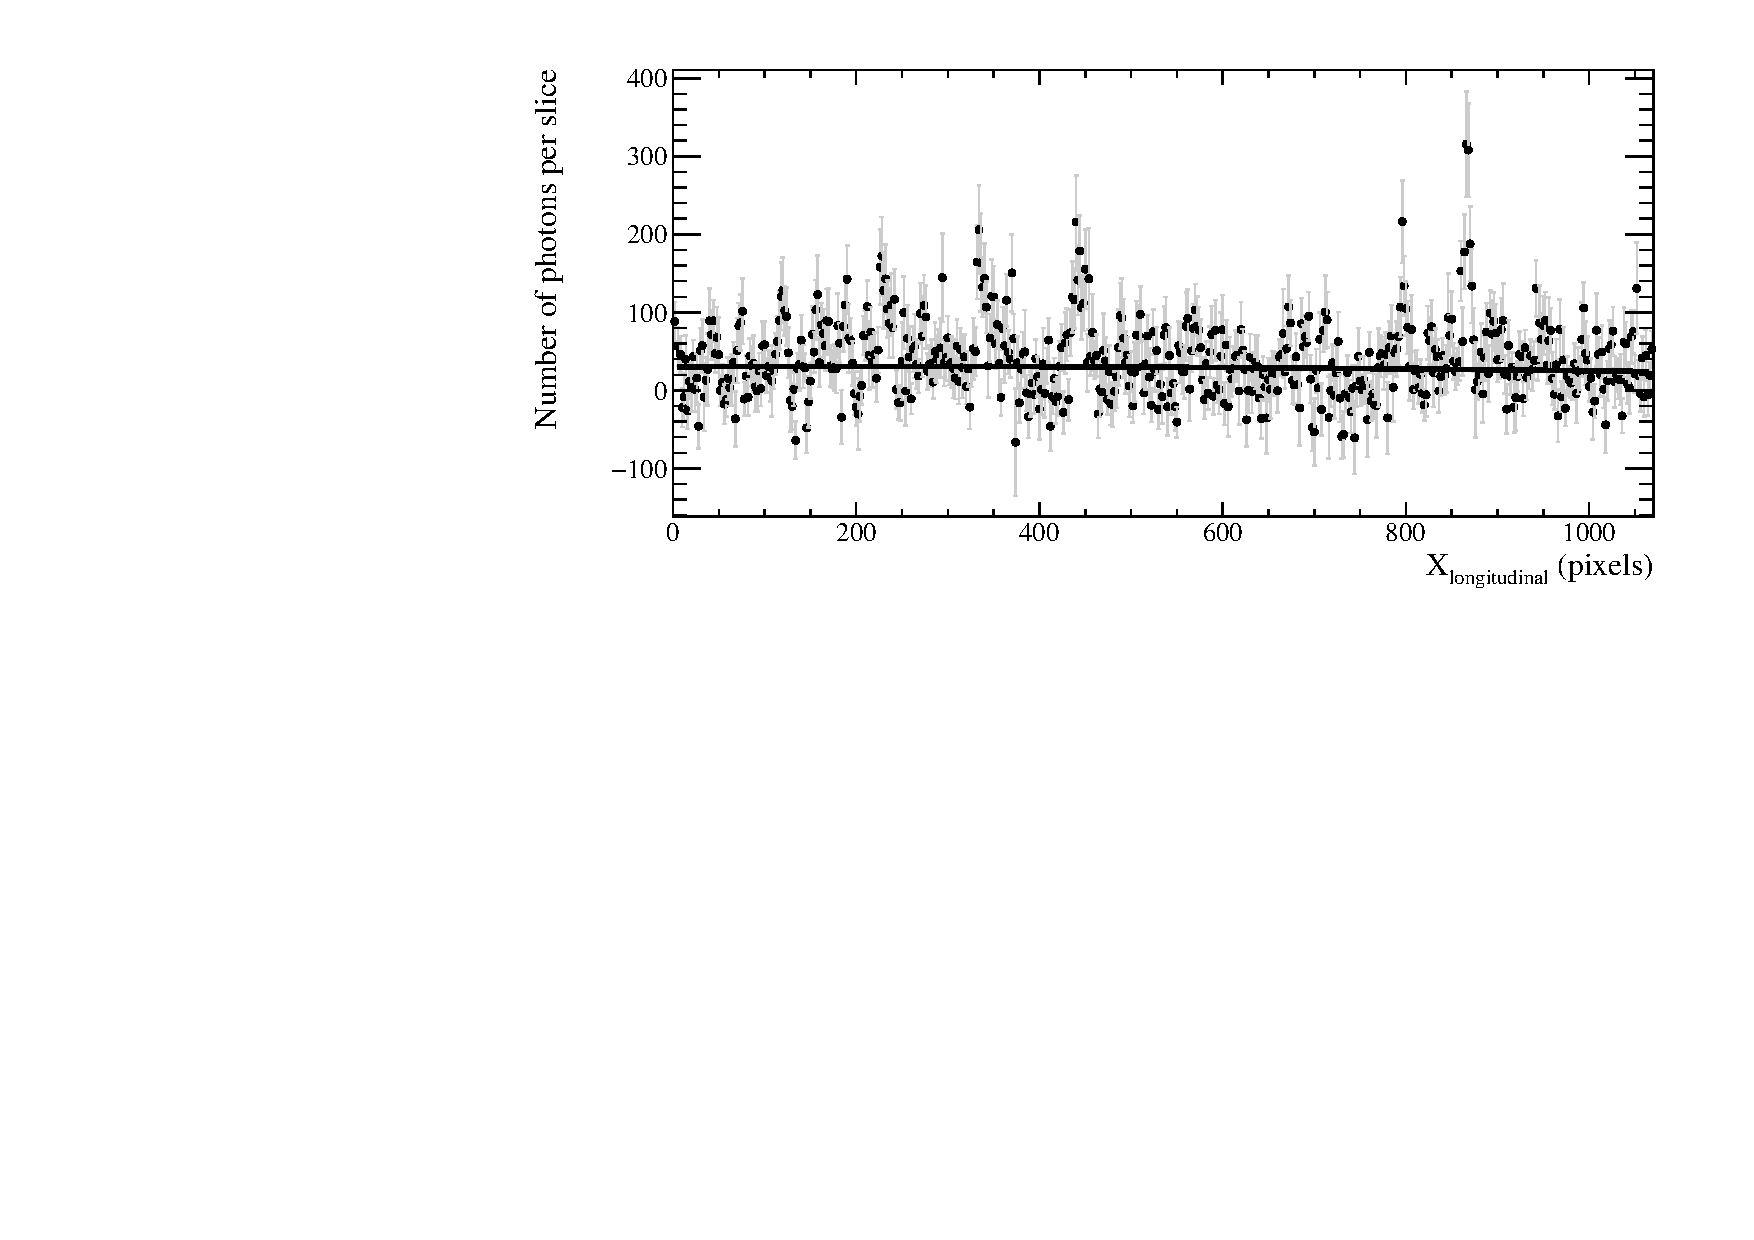
\includegraphics[width=0.45\linewidth]{figures/pic_run02156_ev631_cluster1_longprofile}
        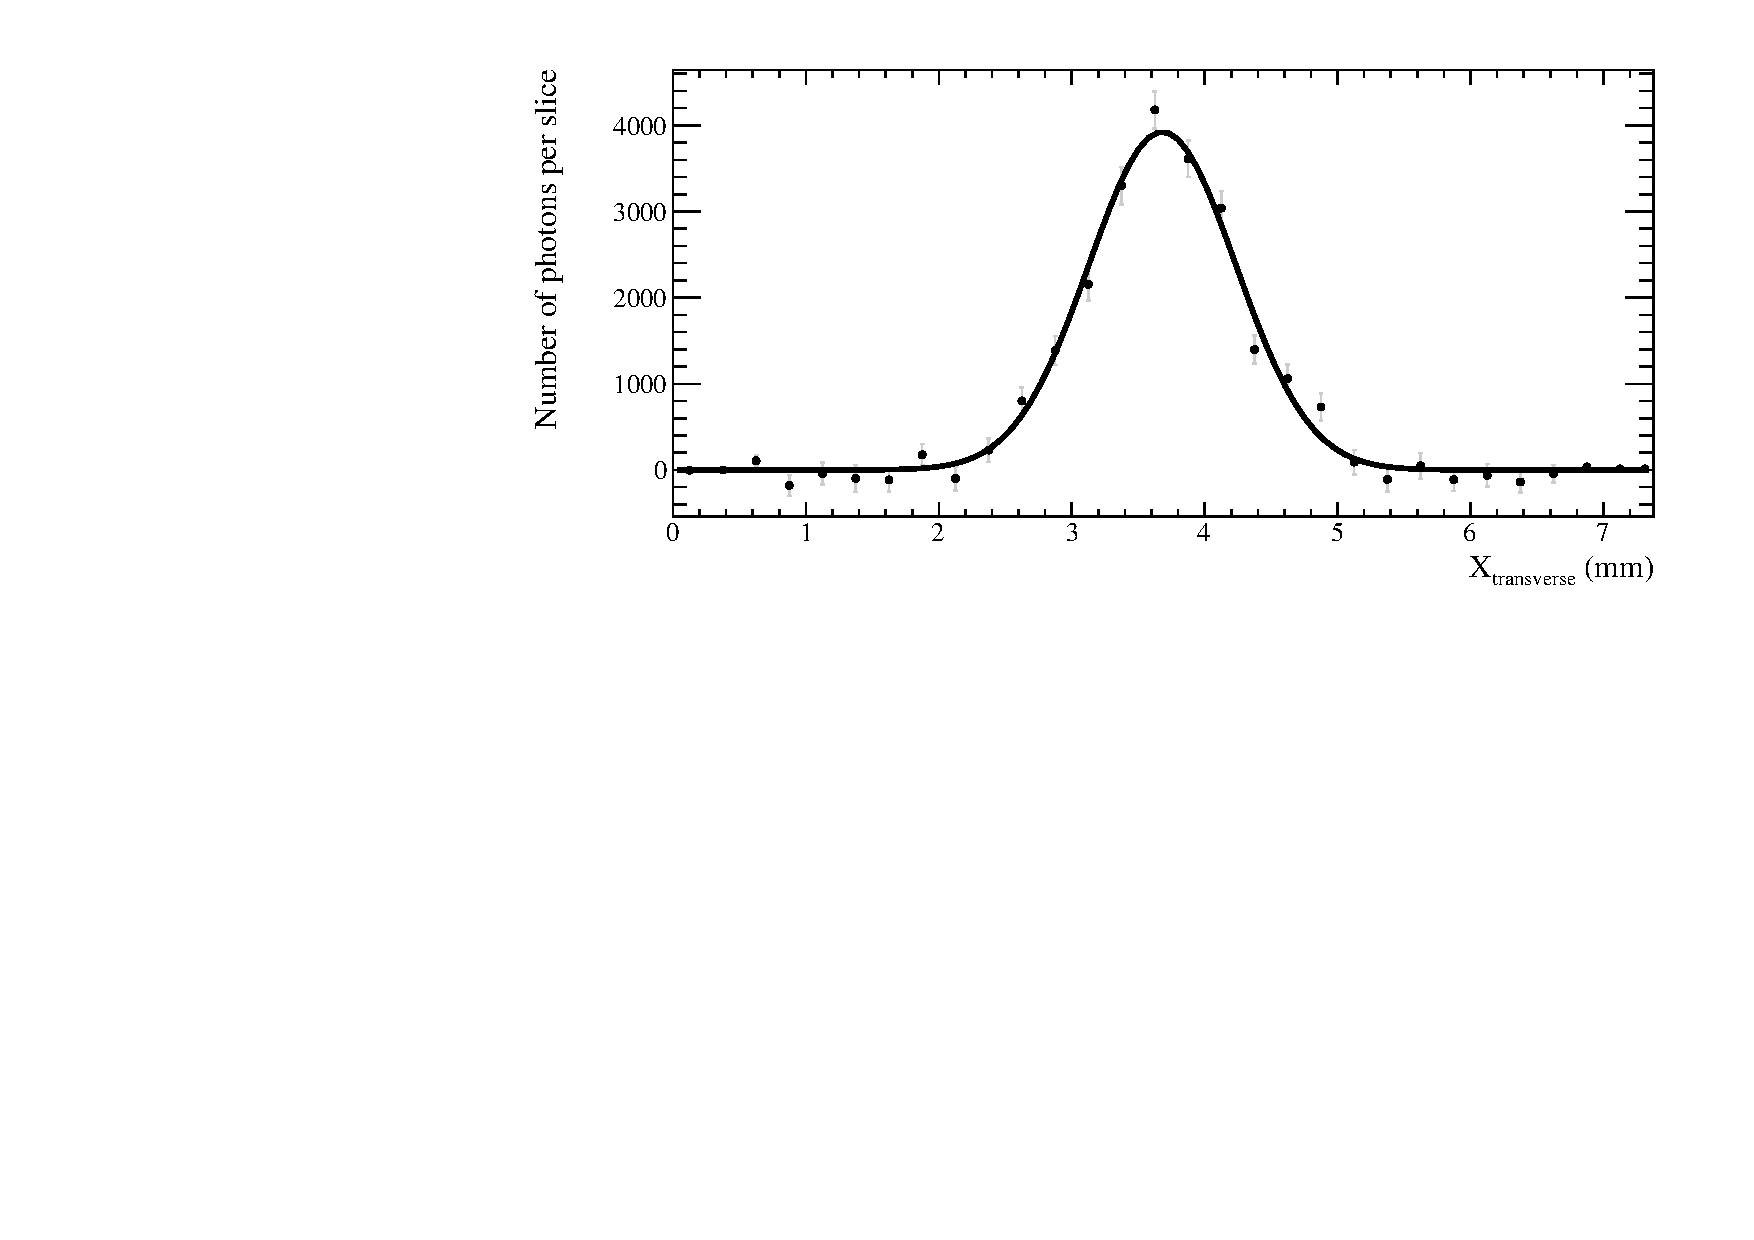
\includegraphics[width=0.45\linewidth]{figures/pic_run02156_ev631_cluster1_latprofile}
        \caption{Supercluster profile in the longitudinal (left) or
          transverse (right) direction, for a long and straight cosmic
          ray track candidate shown in Fig.~\ref{fig:super_clusters2}
          (bottom). The longitudinal profile shows an energy
          deposition in sub-clusters, while the transverse direction
          shows the typical width of the diffusion in the gas. For the
          longitudinal profile, the line represent the average number
          of photons per slice. For the transverse profile, it
          represents a fit with a Gaussian
          PDF. \label{fig:profiles}}
      \end{center}
  \end{figure}

  \item \textit{projected path length:~} for curly and kinky tracks
    the values returned by the SVD of the supercluster are not an
    accurate estimates of their size. While the width is dominated by
    the diffusion, the length for patterns like the one shown in the
    example of Fig.~\ref{fig:super_clusters1} is ill-defined. Thus,
    the more general path length, $l_p$, computed with the
    skeletonization procedure in Fig.~\ref{fig:skeleton} is used to
    estimate the linear extent for both straight and curved tracks.

  \item \textit{Gaussian width:~} the original width of the track in
    the transverse direction is expected to be much lower than the
    observed width induced by the diffusion in the gas. Thus, as shown
    in Fig.~\ref{fig:profiles} (right), the standard
    deviation, \tsigmag, can estimated by a fit with a Gaussian
    probability density function (PDF). This modelling is appropriate
    for the cases of straight tracks, typical of cosmic-ray
    background, or energetic nuclear recoils, and also for spot-like
    clusters. Tracks with kinks are badly modeled by a Gaussian
    function: if the $\chi^2$ of the convergence of the fit is below a
    threshold, the estimated width from the SVD method described
    earlier is used;

  \item \textit{slimness:~} the ratio of the width over the path
    length, $\xi=w/l_p$, represents the aspect ratio of the
    cluster. It is very useful to discriminate between cosmic
    rays-induced background (long and thin) from low energy nuclear or
    electron recoils (more elliptical or round, as the \fe spots);
    
  \item \textit{integral:~} the total number of photons detected by all the
  pixels gathered in the supercluster, \isclu, as defined in
  Eq.~\ref{eq:integral};

  \item \textit{pixels over threshold:~} the number of pixels in the
  supercluster passing the zero-suppression threshold, $n_p$;

  \item \textit{density:~} the ratio $\delta$ of \isclu, divided by
  $n_p$, as defined in Eq.~\ref{eq:density};

  \item \textit{energy:~} the calibrated energy, expressed in keV. The
    calibration method simultaneously performs both the per-slice
    correction as a function of the local $\delta$, and the absolute
    energy scale calibration, which corrects the non perfect
    containment of the cluster, \ie, the bias in the distribution of
    $E/E_{true}$, using with \fe source.
\end{itemize}

The distributions of the projected supercluster path length, $l_p$,
and Gaussian transverse size, \tsigmag, are shown in
Fig.~\ref{fig:clsize}, for data taken in different types of runs.
During the data-taking approximately 3000 frames were recorded in
absence of any external radioactive source ({\it no-source}
sample). In these frames the interaction of ultra-relativistic cosmic
ray particles (mostly muons) are clearly visible as very long
clusters. Internal radioactivity of the \lemon materials also
contributes with several smaller size clusters. About 1500 frames were
acquired with the \ambe source, and approximately $10^4$ calibration
images with \fe source. In Fig.~\ref{fig:clsize}, as well as in the
following ones showing other cluster properties, the distributions
obtained in runs without radioactive sources are normalized to
the \ambe data total CMOS exposure time. For the data with \fe source,
since the activity of the source is such to produce about 15
clusters/event, the data are scaled by a factor one-tenth with respect
to the \ambe exposure time for clearness. Tracks originating from
cosmic-rays interactions are present also in the data with both types
of radioactive sources, with an efficiency scale factor slightly
different from unity because of the trigger. Considerations about the
trigger efficiency, affecting the background normalization in data
with a radioactive source are given in Sec.~\ref{sec:background}. The
distributions in this section aim to show the different cluster shape
observables among the different kinds of events.

\begin{figure}[ht]
  \begin{center}
  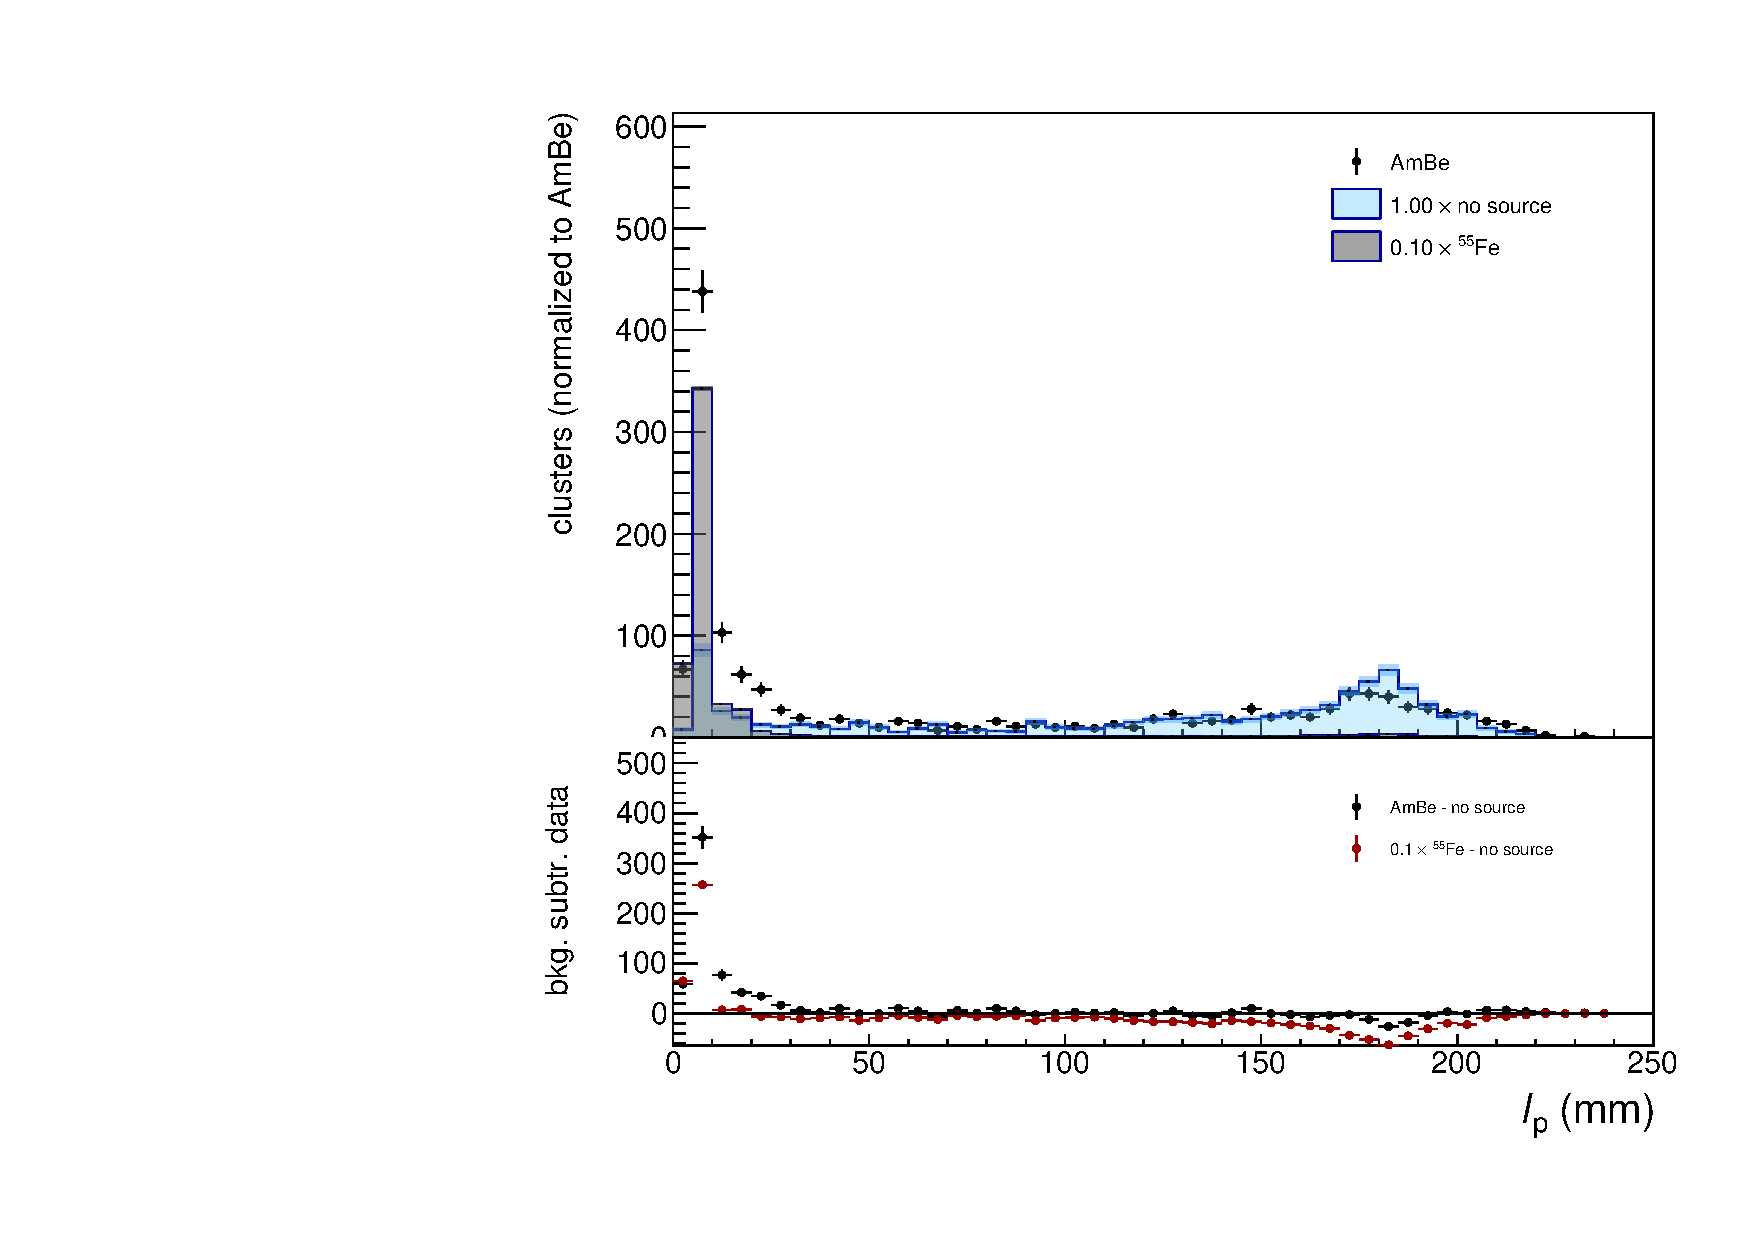
\includegraphics[width=0.45\linewidth]{figures/length}
  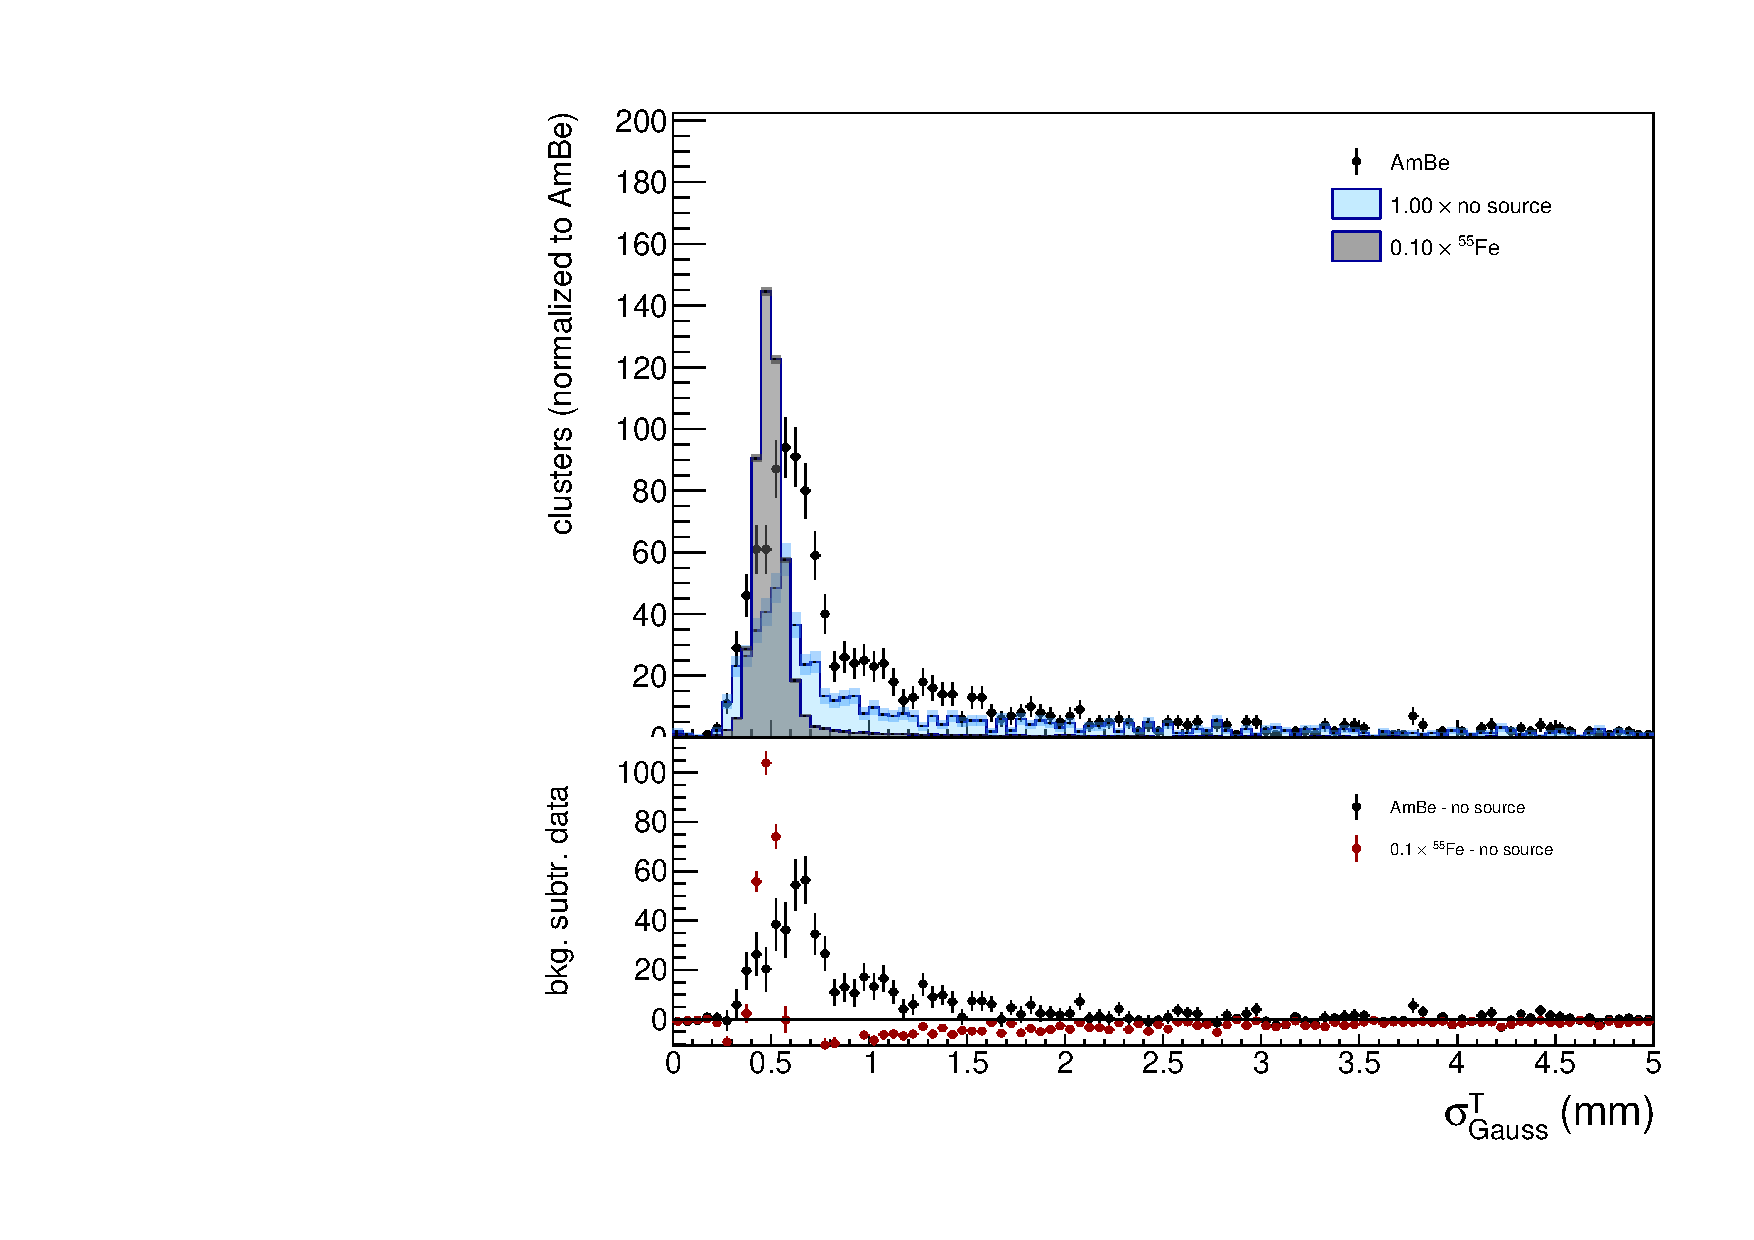
\includegraphics[width=0.45\linewidth]{figures/tgausssigma}

  \caption{Supercluster sizes projected onto the $x$--$y$ plane. Left:
    longitudinal path length, $l_p$.  Right: transverse Gaussian
    spread, \tsigmag. Filled points represent data with \ambe source,
    dark gray (light blue) distribution represents data with \fe
    source (no source).  The normalization of data without any
    radioactive source is scaled to the same exposure time of
    the \ambe one. For the data with \fe source , a scaling factor of
    one tenth is applied for clearness, given the larger activity of
    this source.  \label{fig:clsize}}

    \end{center}
\end{figure}

Figure~\ref{fig:clsize} shows the cluster sizes distributions in the
longitudinal and transverse directions for different sets of
runs. Data show an average Gaussian width for the \fe spots
$\tsigmag\approx500$\unit{$\mu$m} (dominated by the diffusion in the
gas), while it is larger, approximately 625\unit{$\mu$m}, for data
with \ambe source.  The contribution of cosmic rays, present in all
the data, is clearly visible in the data without any radioactive
source, corresponding to clusters with a length similar to the
detector transverse size (22\unit{cm}).

Other observables are the slimness, $\xi$, and the light density,
$\delta$, shown in Fig.~\ref{fig:clshape}. The former is a useful
handle to reject tracks from cosmic rays, which typically have a slim
aspect ratio, \ie, low values of $\xi$, while the clusters from \fe
are almost round, with values $0.9\lesssim\xi<1$. By construction,
$\xi<1$, since the width is computed along the minor axis of the
cluster, and for round spots it peaks at around 0.9. The apparent
threshold effect is purely geometrical, due to the minimal size of the
macro-pixel ($4{\times}4$) used at the basic clustering step which can
be larger than a round spot from \fe. Data with \ambe source, which
contains a component of nuclear recoils, show a component of round
spots, similar in size to the ones of \fe, and a more elliptical
component, with $0.4<\xi<0.8$ values. Aside from the slightly
different normalization of the cosmic-rays background in the region
dominated by these interactions, $0<\xi<0.3$, which is discussed in
Sec.~\ref{sec:background}, the shape of the distribution shows some
differences. This can be attributed to the cases of clusters induced
by the radiation from the source which may overlap with a long track
from a cosmic ray, changing its shape or, rarely, inducing a track
splitting.  The effect on the following statistical analysis is an
underestimation of the signal efficiency, since a loose selection on
this variable is used to discard cosmic-rays background. Given that
the signal concentrates at values of $\xi \approx 0.9$, this effect is
assumed to be negligible.

Finally, the light density, $\delta$, is the variable expected to
better discriminate among different candidates: cosmic rays induced
background, electron recoils and nuclear recoil candidates. This is
the variable used in this paper for the final particle
identification. The identification results can be improved using
additional cluster shape variables, also profiting of their different
correlations for signal and background clusters, via a multivariate
approach, but in this early analysis a simple cut-based approach is
chosen, for simplicity.

\begin{figure}[ht]
  \begin{center}
  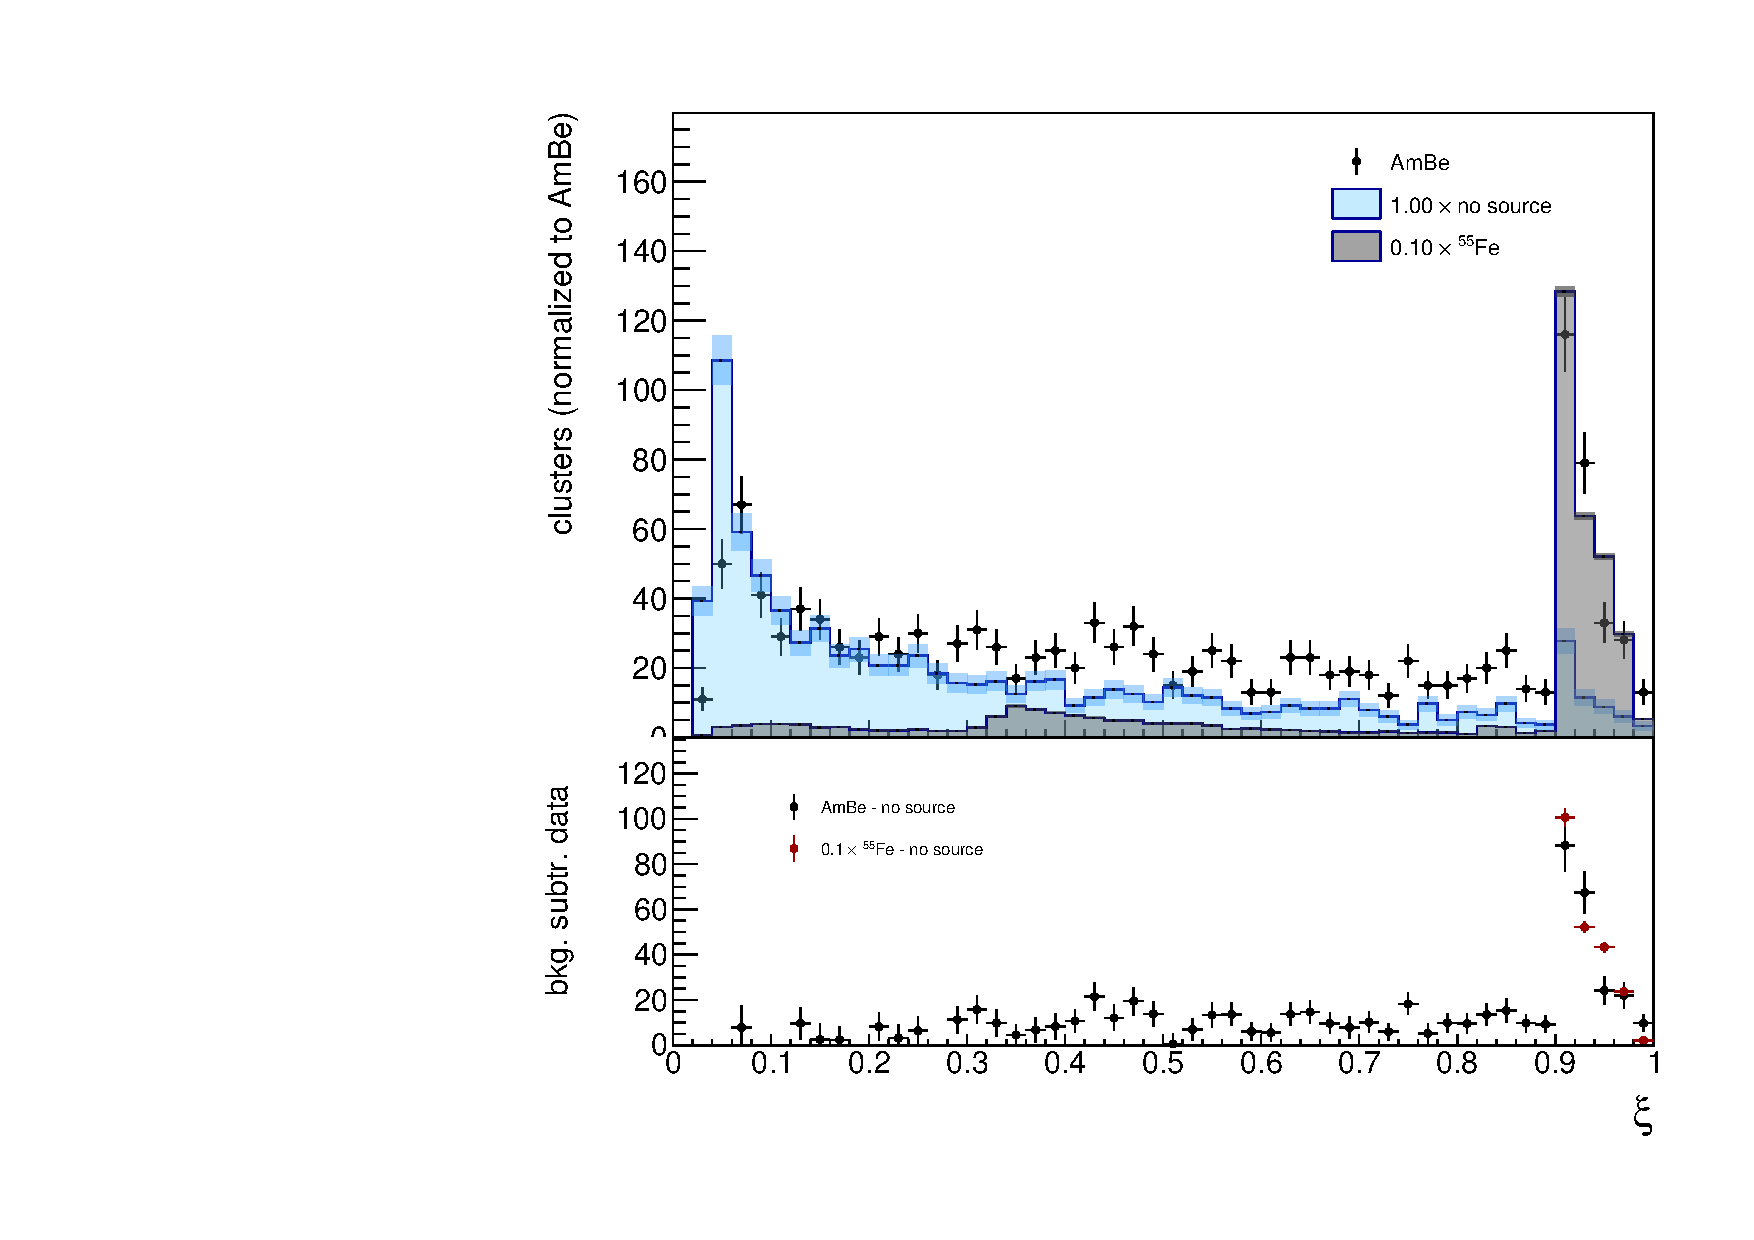
\includegraphics[width=0.45\linewidth]{figures/slimness}
  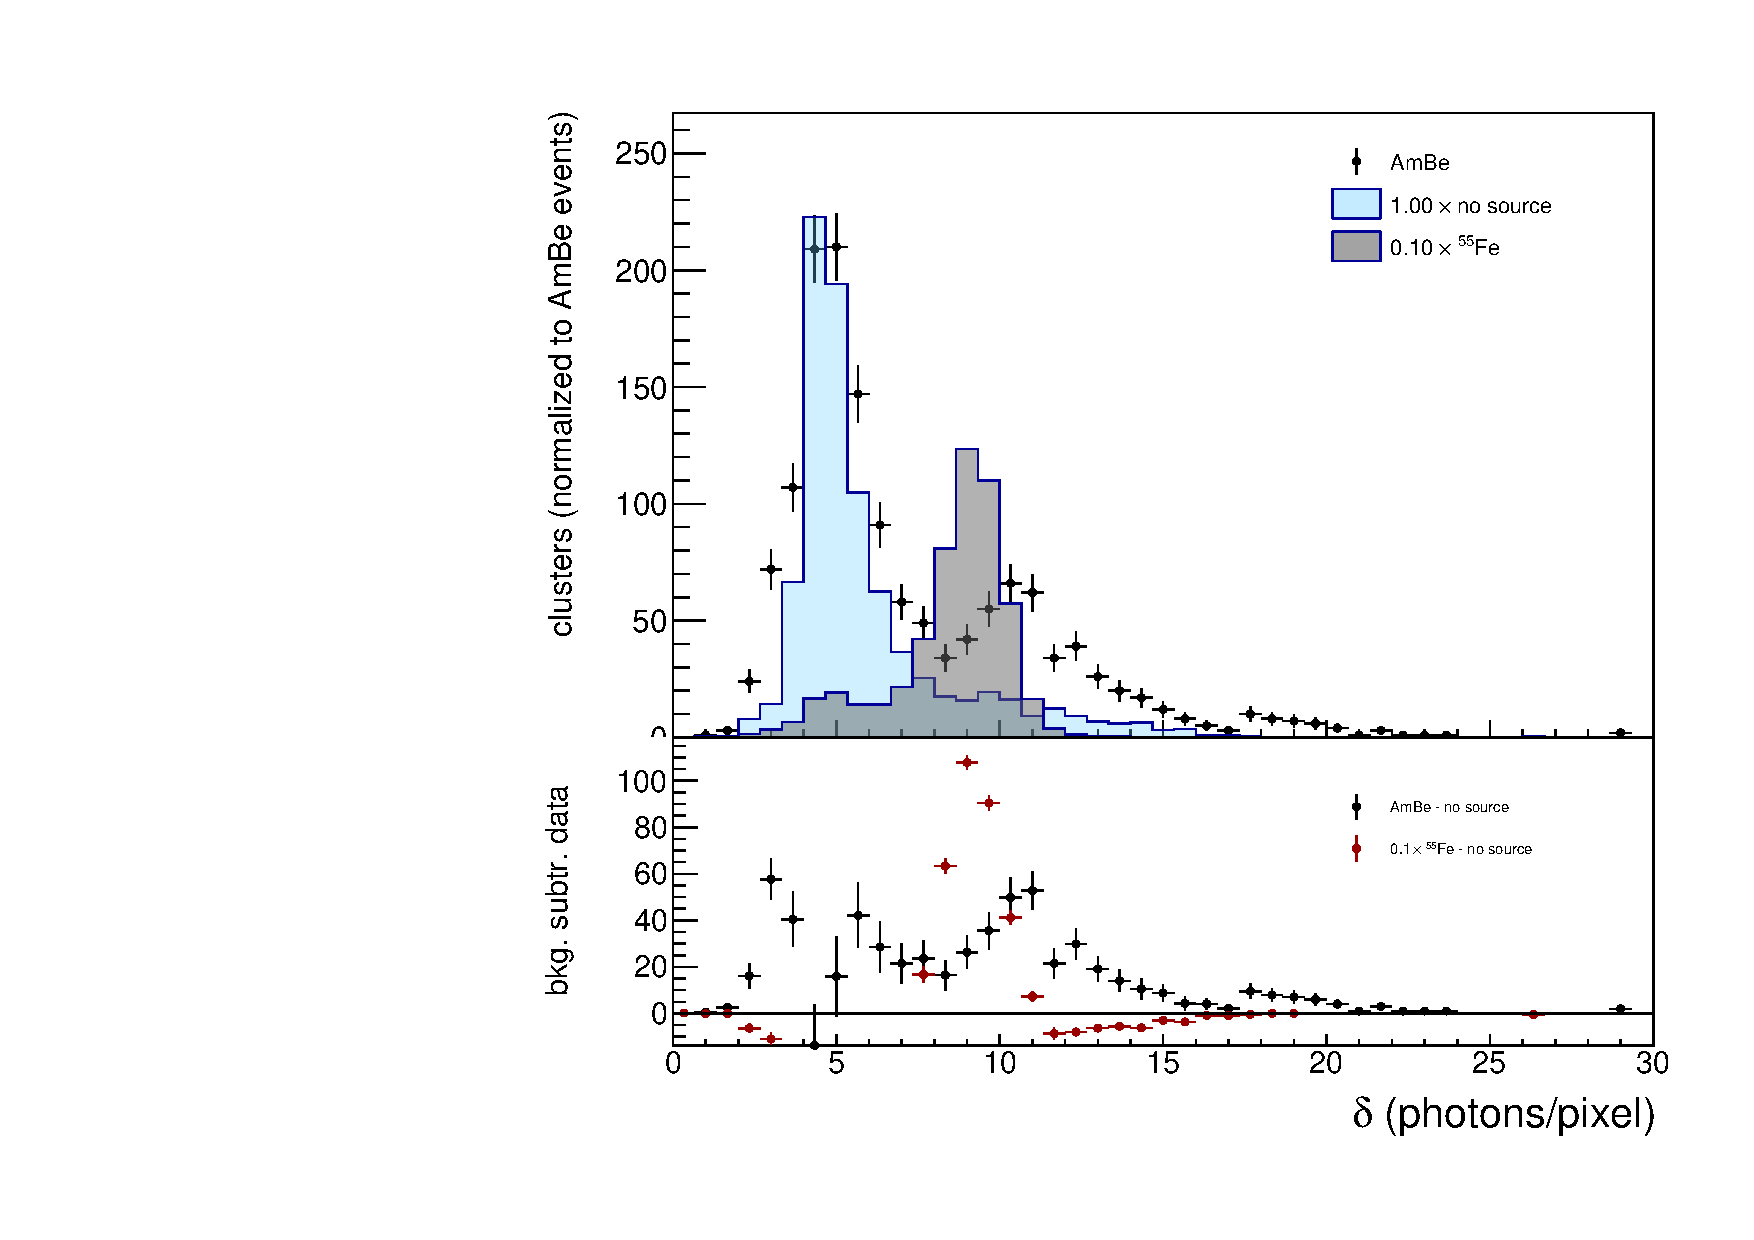
\includegraphics[width=0.45\linewidth]{figures/density}

  \caption{Supercluster variables. Left: slimness $\xi$; right: light
    density $\delta$. Filled points represent data with \ambe source,
    dark gray (light blue) distribution represents data with \fe
    source (no source).  The normalization of data without source is
    to the same exposure time of the \ambe one. For the data with \fe,
    a scaling factor of one tenth is applied for clearness, given the
    larger activity of this source. \label{fig:clshape}}

\end{center}
\end{figure}

Finally, Fig.~\ref{fig:energy} (left) shows the calibrated energy
($E$) spectrum for the reconstructed superclusters. The energy
spectrum shows the $E=5.9\keV$ peak in the first bin of the
distribution for data with \fe source, and the expected broad peak for
minimum ionizing particles traversing the $\approx$20\unit{cm} gas
volume at around 60\keV. The distribution of the observed average
projected \dedl for the no-source sample and for the \ambe samples is
shown in Fig.~\ref{fig:energy} (right). The broadening of the
distribution is mainly due to the specific energy loss fluctuation in
the gas mixture of the cosmic ray particles.  Its modal value,
corrected for the effect of the angular distribution (an average
inclination of 56$^{\circ}$ was measured from track reconstruction) is
2.5\keV/cm, in good agreement with the \garfield prediction of
2.3\keV/cm.

\begin{figure}[ht]
  \begin{center}
  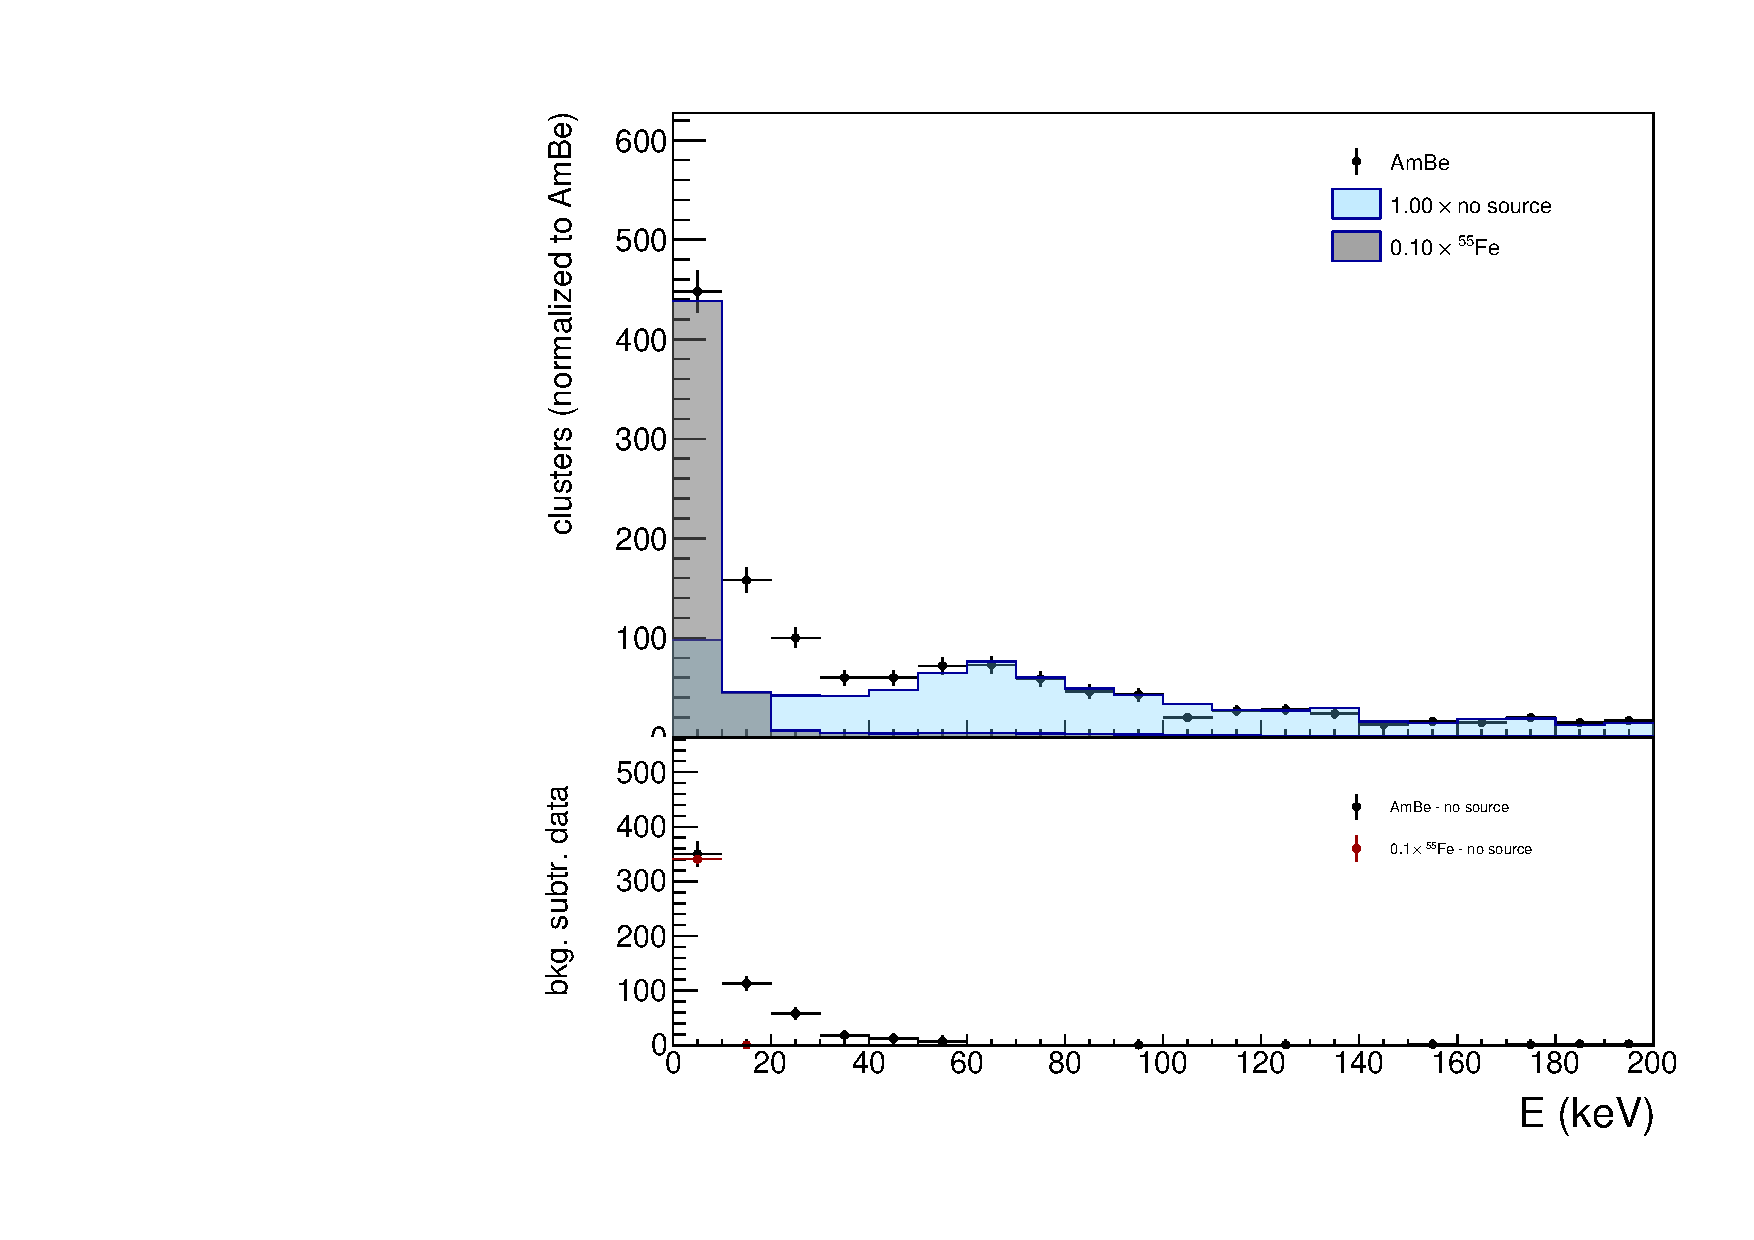
\includegraphics[width=0.45\linewidth]{figures/energyExt}
  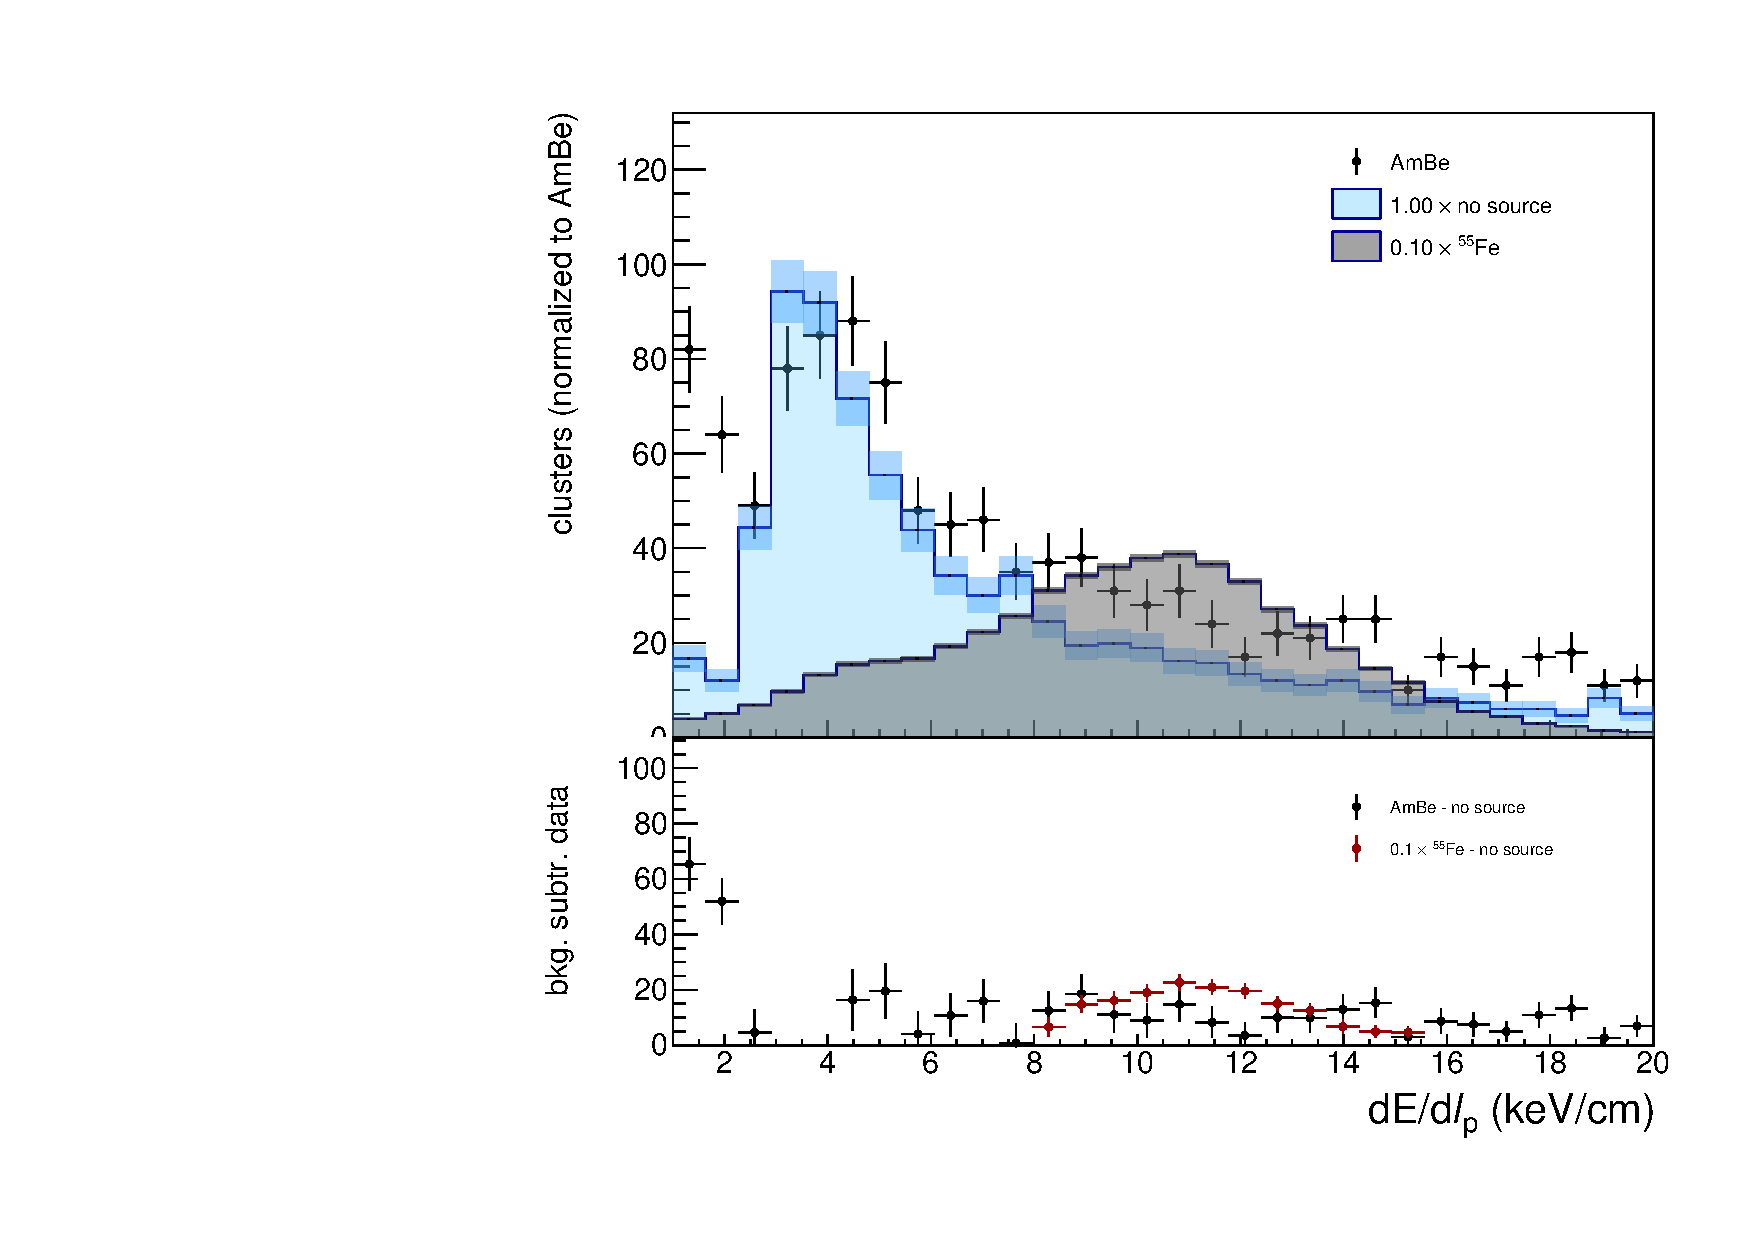
\includegraphics[width=0.45\linewidth]{figures/dedx}

  \caption{Supercluster calibrated energy spectrum (left) and their
    average \dedl. Filled points represent data with \ambe source,
    dark gray (light blue) distribution represents data with \fe
    source (no source).  The normalization of data without source is
    to the same exposure time of the \ambe one. For the data with \fe,
    a scaling factor of one tenth is applied for clearness, given the
    larger activity of this source. \label{fig:energy}}

\end{center}
\end{figure}

\subsection{Background normalization}
\label{sec:background}
The data with \ambe source, taken on the Earth surface, suffers from a
large contribution of interactions of cosmic rays, and from ambient
radioactivity, whose suppression is not optimized for the \lemon
detector. The cluster shape observables provide a powerful handle to
discriminate them from nuclear recoils candidates, but the small
residual background needs to be statistically subtracted. The
distributions shown earlier, where the different types of data are
normalized to the same exposure time, demonstrate that the live-time
normalization provides already a good estimate of the amount of cosmic
rays in data with radioactive sources. This approach does not account
for a possible bias from the trigger, which is generated by the PMT
signals, as described in Sec.~\ref{sec:layout}. Indeed, in runs with
the \ambe source, the PMT can trigger both on signals from neutron
recoils or photons produced by the $^{241}$Am, and on ubiquitous
signals from cosmic rays, while in the sample without source only the
latter are possible.  Therefore, during the same exposure time,
the probability to trigger on cosmic rays is lower in events
with \ambe than in no-source events. The trigger efficiency scale
factor, $\varepsilon_{SF}$, can be obtained as the ratio of the number
of clusters selected in pure control samples of cosmic rays ($CR$)
obtained on both types of runs:
\begin{equation}
\label{eq:sfeff}
\varepsilon_{SF} = \frac{N^{AmBe}_{CR}}{N^{no-source}_{CR}}.
\end{equation}

The $CR$ control region is defined by selecting clusters with
$l>13$\unit{cm}, $\xi<0.1$, $\tsigmag<6$\unit{mm}, and having an
energy within a range dominated by the cosmic rays contribution,
$50<E<80\keV$. The selected clusters show small values of
$\delta\approx5$, well compatible with the small specific ionization
of ultra-relativistic particles.  This sample is limited in
statistics, but it is expected to be almost 100\% pure. The scale
factor obtained is $\varepsilon_{SF}=0.75\pm0.02$.  A possible
consequence of occasional nearby clusters from nuclear recoils
changing the distribution of $\xi$ is considered. The effect is
expected to be reduced for the long clusters selected in the $CR$
control region. A systematic uncertainty due to the different shape of
$\xi$ is estimated by applying the $CR$ selection on the \ambe
clusters where the slimness is substituted, cluster-by-cluster,
sampling the distribution in the no-source data. The difference in the
$N^{AmBe}_{CR}$ is about 1\%, small with respect to the statistical
uncertainty of $\varepsilon_{SF}$.

In addition to the normalization correction of the cosmic-rays
background to be applied before subtracting it to the source data, it
has been mentioned earlier that occasional overlap of long tracks from
this background and signal tracks moderately distort the cluster shape
distributions. Splitting of a long track in the data with the source
may happen because of a gradient change in the region of the overlap
with a dense nuclear recoil cluster. The typical track lengths of
cosmic rays and signal tracks are so different that in these
occurrences the split tracks are still much longer than the signal
ones, thus they are rejected.  In other cases, when the overlap is
close to the edges, the track length is increased, and the selection
dismisses those clusters.  Since the requirement on the track length
is very loose, the effect on the signal efficiency is assumed to be
negligible.

In Fig.~\ref{fig:cosmics} the typical light density and polar angle
(with respect the horizontal axis) distributions for long clusters
selected with the $CR$ requirements, except the energy one are shown
for the \ambe and for the no-source sample, after having applied the
$\varepsilon_{SF}$ scale factor to the latter.  Clusters with
$\delta<6$ are thus expected to be mostly coming from muon tracks, and
they show indeed a polar angle which is shifted at values towards
$90^\circ$.


\begin{figure}[ht]
  \begin{center}
  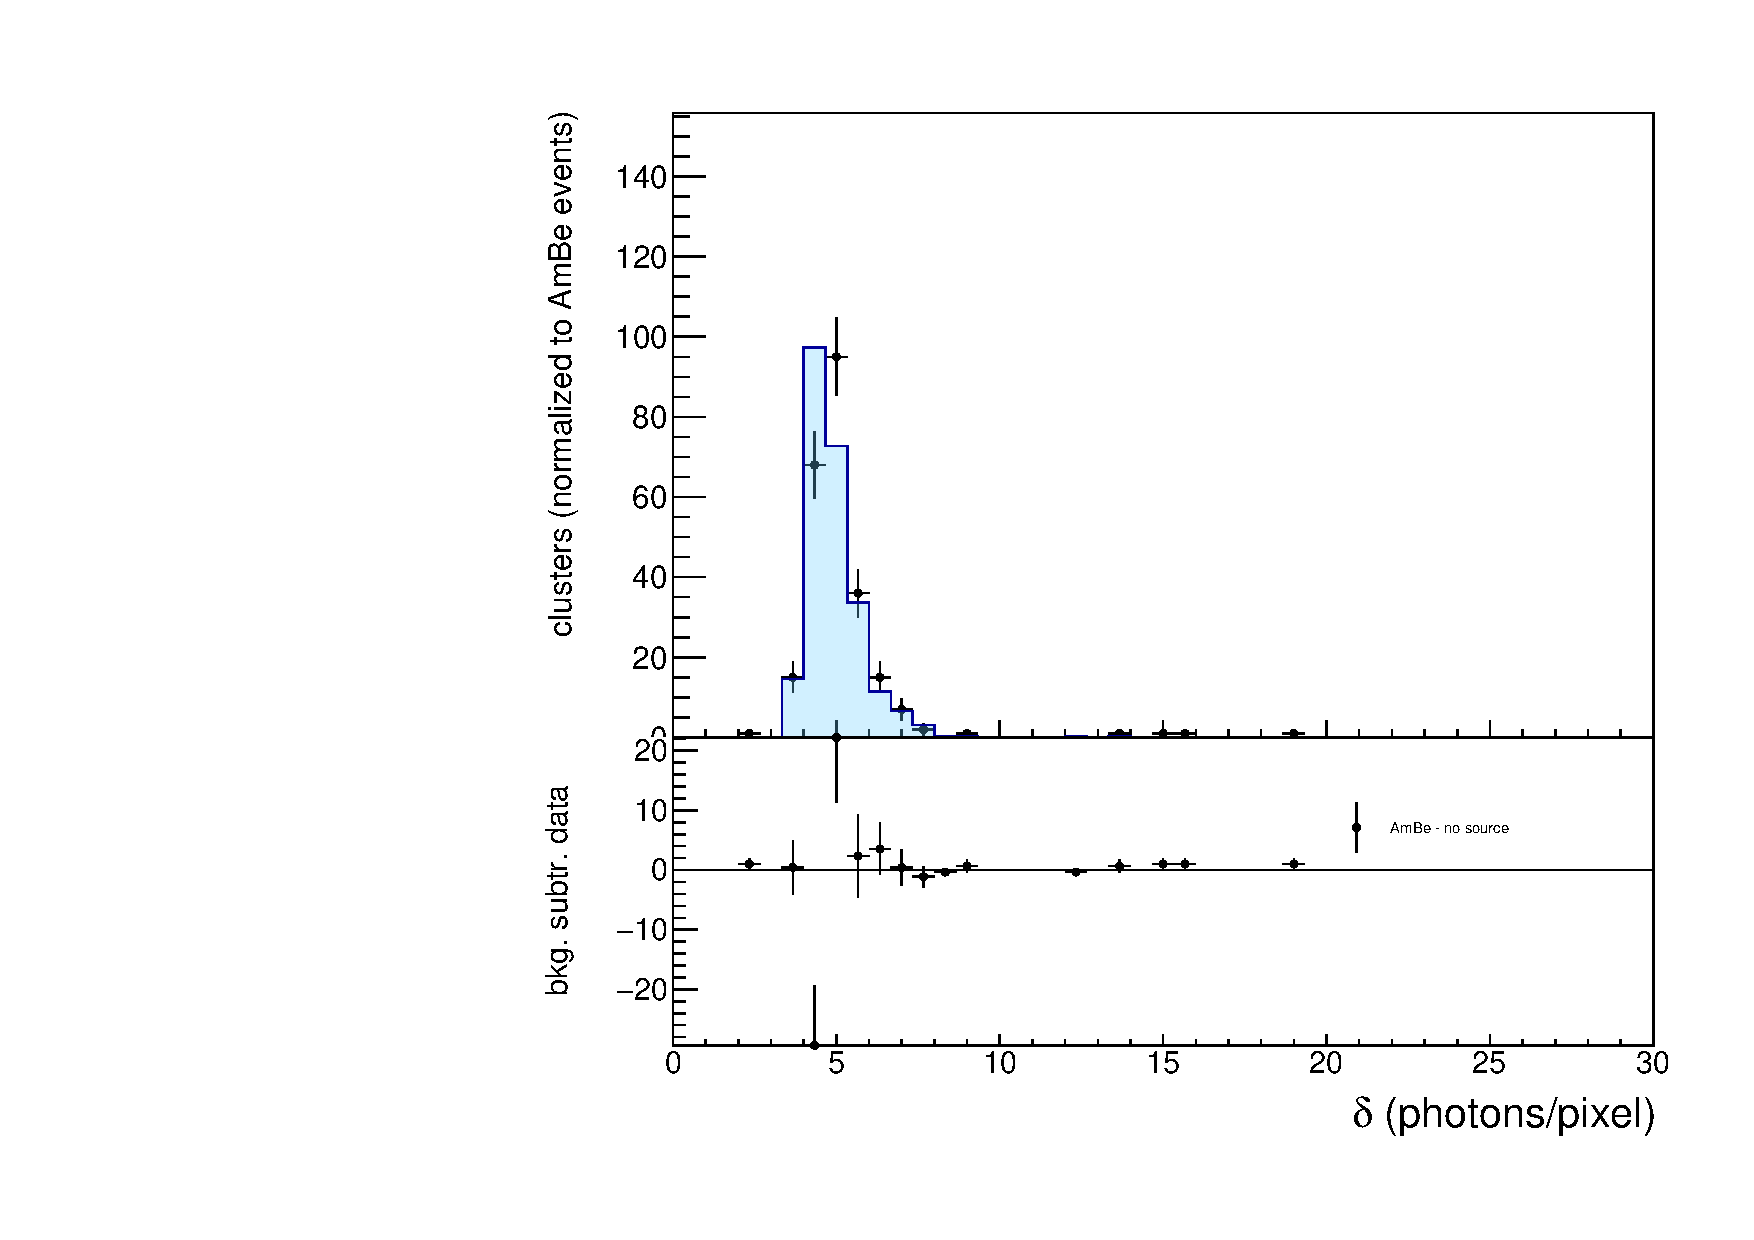
\includegraphics[width=0.45\linewidth]{figures/density_cosmics}
  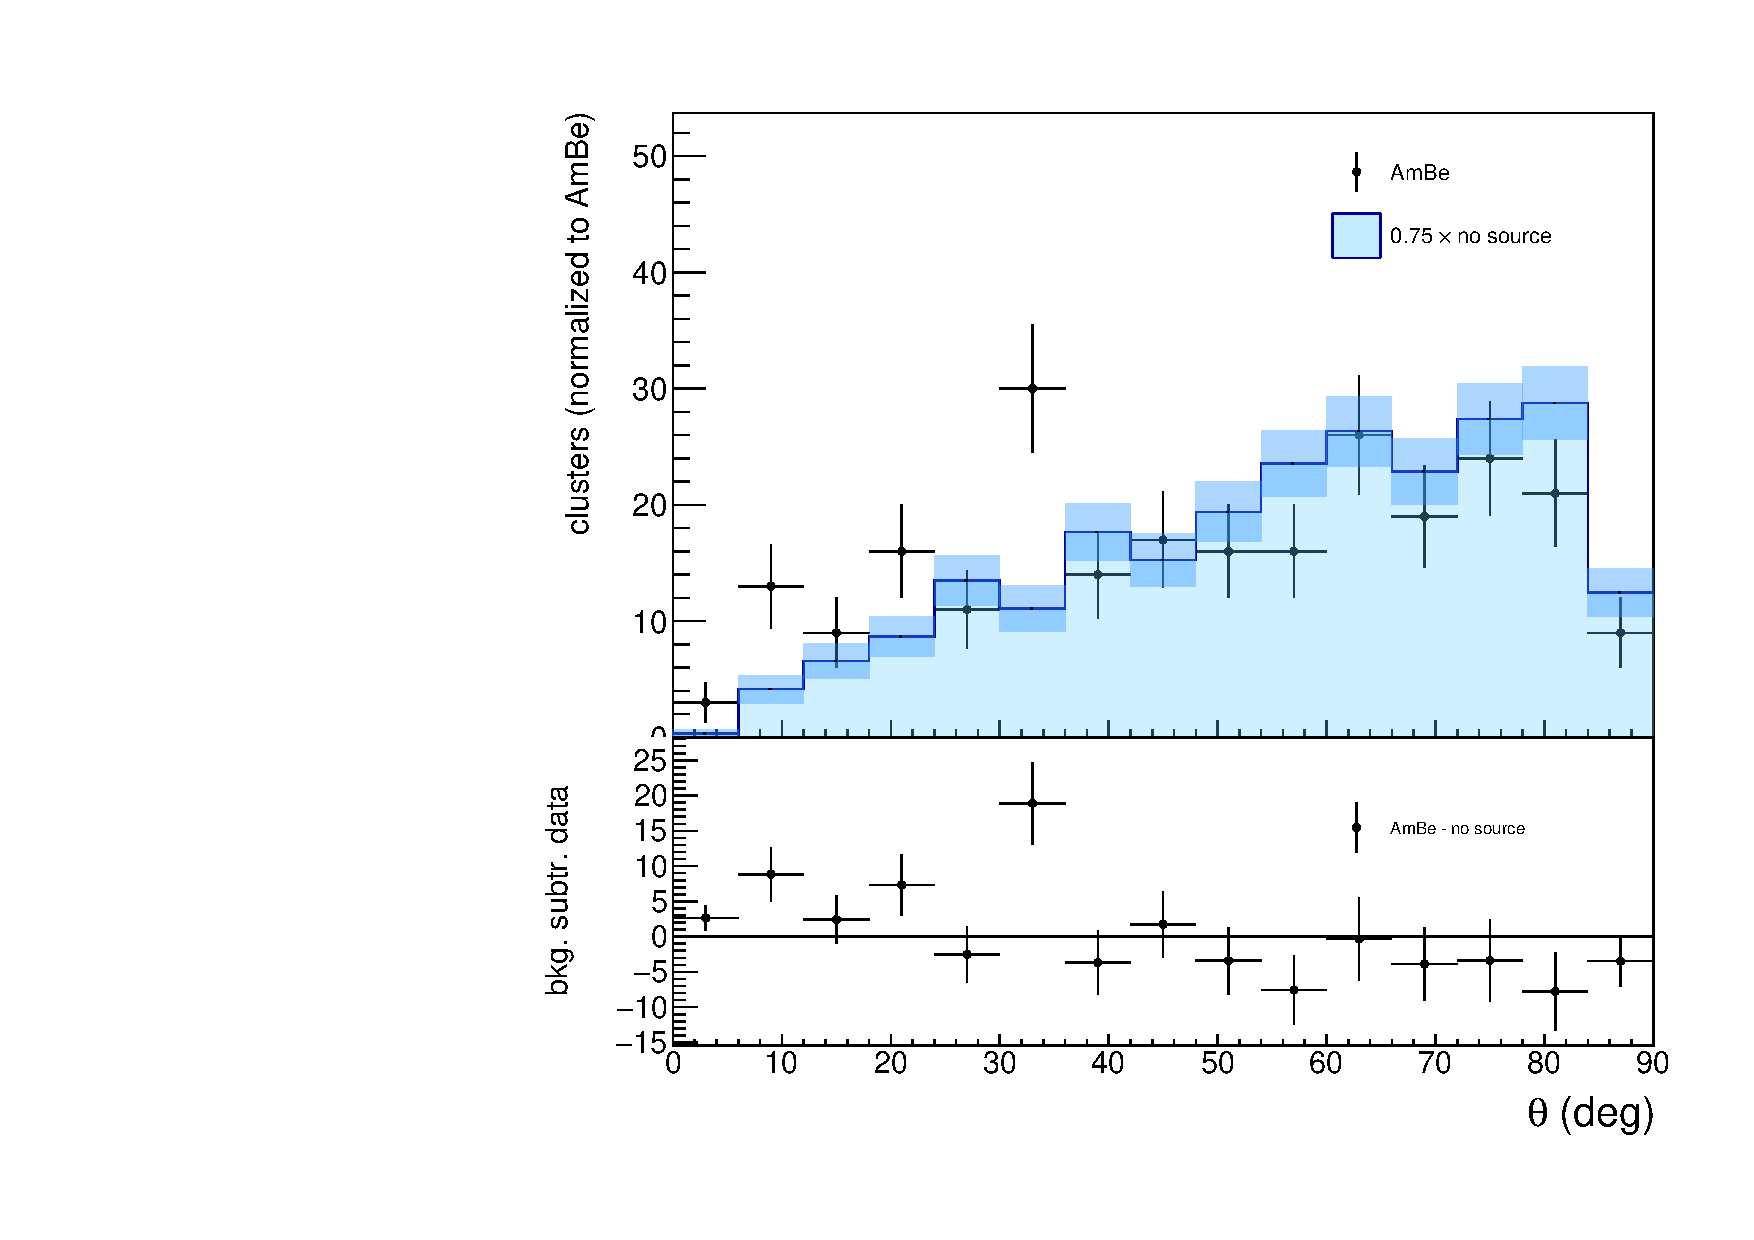
\includegraphics[width=0.45\linewidth]{figures/inclination_cosmics}

  \caption{Supercluster light density $\delta$ (left) and polar angle
    (right) - with respect the horizontal axis - distributions for
    long clusters, dominated by cosmic rays tracks. The clusters are
    selected by the $CR$ requirements, except the energy one.  Filled
    points represent data with \ambe source, light blue distribution
    represents data without any radioactive source.  The normalization
    of data without source is to the same exposure time of the \ambe
    one, accounting for the trigger scale factor $\varepsilon_{SF}$,
    as defined in the text. Bins with negative contents are set to
    zero value. \label{fig:cosmics}}

\end{center}
\end{figure}
